\documentclass[border=12pt]{standalone}
\usepackage{pgfplots}
\pgfplotsset{compat=1.8}

\begin{document}
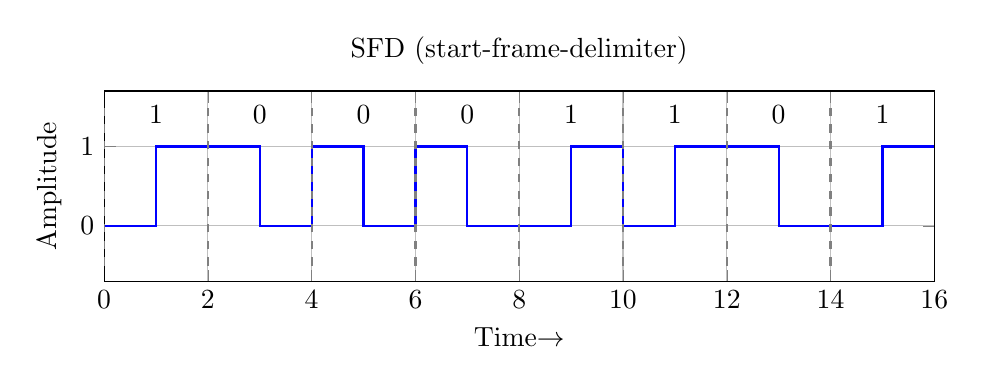
\begin{tikzpicture}
    \begin{axis}[grid=both,xmin=0,xmax=16,width=\textwidth,height=4cm,
        title=SFD (start-frame-delimiter),xlabel={Time$\rightarrow$},ylabel=Amplitude]
        \newcounter{graphStep}
        \setcounter{graphStep}{0}
        \newcounter{prevNumber}
        \setcounter{prevNumber}{0}
        \pgfplotsinvokeforeach{1,0,0,0,1,1,0,1} {
            \edef\bin{\noexpand\node[] at (axis cs: \arabic{graphStep}*2+1,1.40) { #1 };}
            \bin

            \ifnum \value{graphStep} > 0
                \ifnum #1 = 0
                    \ifnum \value{prevNumber} = 0
                        \addplot+[thick,blue,solid,no marks]  coordinates { (\value{graphStep}*2,0) (\value{graphStep}*2,1) };
                    \fi
                \else
                    \ifnum \value{prevNumber} = 1
                        \addplot+[thick,blue,solid,no marks]  coordinates { (\value{graphStep}*2,0) (\value{graphStep}*2,1) };
                    \fi
                \fi
            \fi
            \ifnum #1 = 0
                \addplot+[thick,blue,solid,no marks] coordinates {
                    (\number\value{graphStep}*2,1)
                    (\number\value{graphStep}*2+1,1)
                    (\number\value{graphStep}*2+1,0)
                    (\number\value{graphStep}*2+2,0)
                };
            \else
                \addplot+[thick,blue,solid,no marks] coordinates {
                    (\number\value{graphStep}*2,0)
                    (\number\value{graphStep}*2+1,0)
                    (\number\value{graphStep}*2+1,1)
                    (\number\value{graphStep}*2+2,1)
                };
            \fi
            \addplot+[thick,gray,dashed,no marks] coordinates {
                (\number\value{graphStep}*2,-0.5)
                (\number\value{graphStep}*2,1.5)
            };
            \stepcounter{graphStep}
            \setcounter{prevNumber}{#1}
        }
    \end{axis}
\end{tikzpicture}
\end{document}
